\subsection{Thermally driven creep in rock salt}
\label{subsec:Mc2}

\subsubsection{Definition}
\label{subsubsec:Mc2_def}

Several models exists for the evaluation of the effect of stationary creep in rock salt. One of those models is the so-called BGRa-model Eq.~(\ref{Mc_eqn:BGRa_model}), which is valid for an external load between $5\,$Mpa and $25\,$Mpa within a temperature range of $22$-$200^{\circ}\,$C (\cite{HunSchu:94}).
%
\begin{equation}
\miu{\varepsilon}{\mathrm{c}}{\dot}
=
A e^{-\frac{Q}{R T}}
\left( \frac{\sigma}{\sigma^*} \right)^n
\label{Mc_eqn:BGRa_model}
\end{equation}

In a cylindrical sample of rock salt stress relaxation is caused by a temperature decrease of $30\,$K. The aim of the example is to calculate the resulting strain variation with time within the solid body using the stationary creep model BGRa (\ref{Mc_eqn:BGRa_model}). The results of the simulation defining an axisymmetric model are compared to a threedimensional solution.

\subsubsection{Solution}
\label{subsubsec:Mc2_sol}

For the numerical simulation a cylindrical core sample as shown in Fig.~\ref{Mc_fig:creep_salt_1} is selected.
%
\begin{figure}[htb]
\centering
\includegraphics[scale=0.8]{PART_II/M/creep_salt_1}
\caption{Core sample model}
\label{Mc_fig:creep_salt_1}
\end{figure}

Fig.~\ref{Mc_fig:creep_salt_2} shows the axisymmetric finite element model (mesh, boundary conditions etc.) arranged in the $x$-$z$-plane. The dimensions of this model are: radius ($x$-direction) $0.05\,$m and height $0.2\,$m. A relatively coarse mesh consisting of 228 triangular elements and 139 nodes is used.
%
\begin{figure}[htb]
\centering
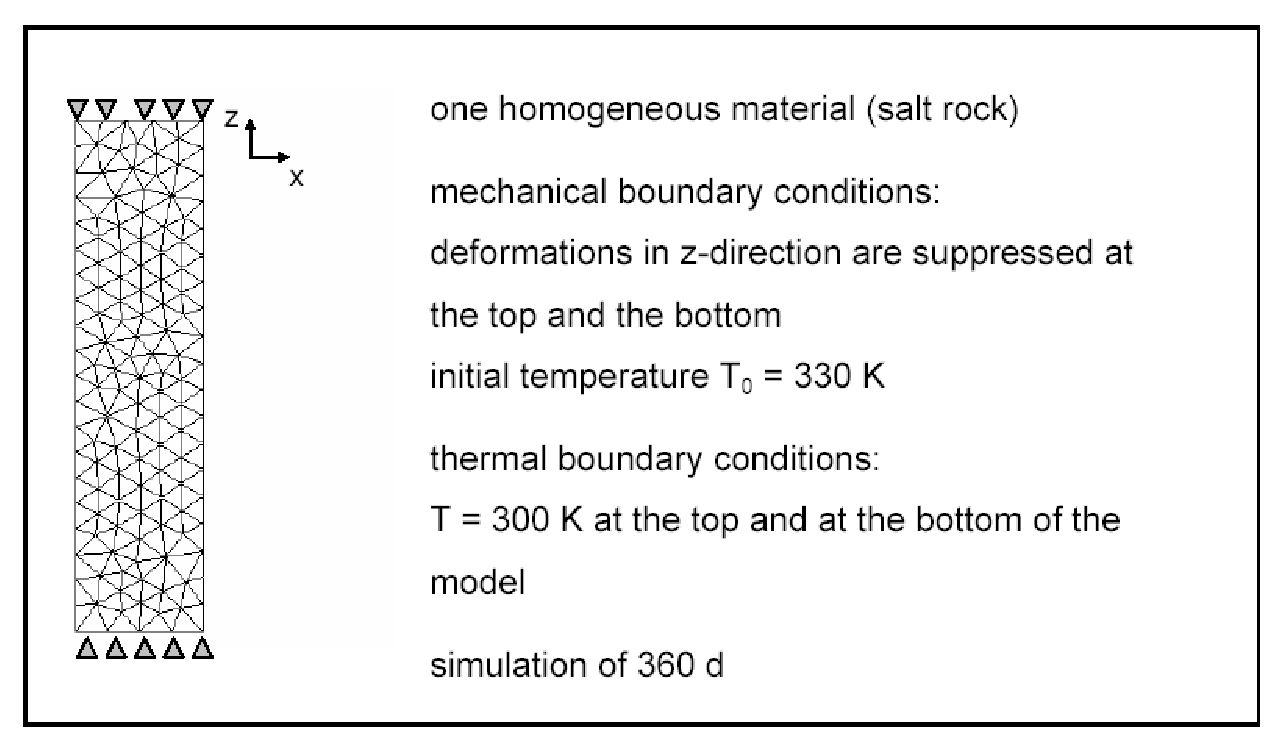
\includegraphics[scale=0.5]{PART_II/M/creep_salt_2}
\caption{Details of the axisymmetric finite element model} \label{Mc_fig:creep_salt_2}
\end{figure}

Vertical deformation at the top and the bottom surfaces are suppressed. The initial temperature in the
whole area is $330\,$K. At the top and the bottom of the model thermal boundary conditions are prescribed defining a temperature of $300\,$K. Based on these conditions, the stress relaxation during the cooling down is simulated.

The material parameters referred to the creep model Eq.~(\ref{Mc_eqn:BGRa_model}) are presented in Table~\ref{Mc_tab:creep_salt}.
%
\begin{table}[!htb]
\centering
\caption{Material parameters of the creep model}
\label{Mc_tab:creep_salt}
\begin{tabular}{llll}
\toprule
Symbol & Parameter & Value & Unit \\
\midrule
$A$        & Factor of the creep model  & $0.18$    & d$^{-1}$                        \\
$Q$        & Activation energy          & $54$      & kJ$\cdot$mol$^{-1}$             \\
$R$        & Gas constant               & $8.31447$ & J$\cdot$K$^{-1}\cdot$mol$^{-1}$ \\
$n$        & Material constant          & $5$       & --                              \\
$\sigma^*$ & Reference effective stress & $1$       & MPa                             \\
\bottomrule
\end{tabular}
\end{table}

In Table~\ref{Mc_tab:creep_salt_heat}, material and process parameters of the thermo-elastic part of the constitutive model are given.
%
\begin{table}[!htb]
\centering
\caption{Material parameters and heat process conditions of the thermo-mechanical creep model}
\label{Mc_tab:creep_salt_heat}
\begin{tabular}{llll}
\toprule
Symbol & Parameter & Value & Unit \\
\midrule
$E$       & Young's modulus                & $25$                & GPa                            \\
$\nu$     & Poisson's ratio                & $0.27$              & --                             \\
$\alpha$  & Thermal expansion coefficient  & $4.0\times 10^{-5}$ & K$^{-1}$                       \\
$c$       & Thermal capacity               & $1$                 & J$\cdot$kg$^{-1}\cdot$K$^{-1}$ \\
$\lambda$ & Thermal conductivity           & $100$               & W$\cdot$m$^{-1}\cdot$K$^{-1}$  \\
\cmidrule{1-4}
$T_0$     & Initial temperature            & $330$               & K                              \\
$T$       & Temperature after cooling down & $300$               & K                              \\
\bottomrule
\end{tabular}
\end{table}

The numerical simulation of the stress relaxation process over a time of $360\,$days is performed within 360 time steps of constant time step length.

In order to evaluate the numerical results of the relaxation problem, the following analytical solution of Eq.~(\ref{Mc_eqn:BGRa_model}) for the problem under consideration has been proposed (Eickemeier 2007, personal communication) in respect of the stress increment for the current time step:
%
\begin{equation}
\Delta\sigma_{i+1}
=
\frac
{(\mib{\varepsilon}{0}{\mathrm{c}}{\dot} - A (\sigma/\sigma^*)^n) E_q \Delta t}
{1 - E_q / \sigma^* A^* \Delta t\,\xi\,n\,(\sigma/\sigma^*)^{n-1}}
\label{Mc_eqn:BGRa_model_2}
\end{equation}
%
with
%
\begin{equation}
A^*
=
A e^{-Q/RT}
\label{Mc_eqn:BGRa_model_3}
\end{equation}
%
Here, the initial creep strain rate $\mib{\varepsilon}{0}{\mathrm{c}}{\dot}$ is assumed to be zero, $E_q$ is the weighted Young's modulus of the steel plates, which are used to apply the external load and to support the sample, and the rock salt sample (in this case, only rock salt is considered), and the paramter $\xi$ is defined as $\xi=0.5$.

\subsubsection{Results}
\label{subsubsec:Mc2_res}

For the analytical solution of Eq.~(\ref{Mc_eqn:BGRa_model_2}) the axial stress of the previous time step is used. Time step increment is $\Delta t= 1\,$d. In the threedimensional case, the results are shown for node 705, which is located at point $(x,\,y,\,z=0.05,\,0,\,0.12)$. This node is identical to node 76 of the axisymmetric model (cf. Fig.~\ref{Mc_fig:creep_salt_3}).

The comparison of the increment of axial stresses $\Delta\sigma_{i+1}$ analytically obtained using Eq.~(\ref{Mc_eqn:BGRa_model_2}) shows identical results to the numerical values at node 705 of the threedimensional model and node 76 of the axisymmetric model. Both stress increments $\Delta\sigma_{i+1}$
obtained by OpenGeoSys and the scientific special purpose finite element code ANSALT (cf. \cite{GHKN:1995}) are equal to $3.05\times 10^{-3}\,$MPa. The results of axisymmetric as well as threedimensional numerical simulations are shown in Fig.~\ref{Mc_fig:creep_salt_3}, and show an excellent agreement.
%
\begin{figure}[htb]
\centering
\includegraphics[scale=0.28]{PART_II/M/creep_salt_3}
\caption{Comparison of numerical results (OpenGeoSys vs. ANSALT) for axial stresses}
\label{Mc_fig:creep_salt_3}
\end{figure}
